\section{Design}
\subsection{UI Design}
Bevor mit der Entwicklung des Frontends begonnen werden kann, muss geplant werden, wie dieses aussehen soll. Um ein möglichst gutes Ergebnis zu erzielen, ist es wichtig sich folgende Fragen zu stellen \footcite{ui_design_questions}:

\begin{itemize}
	\item Welche Anforderungen werden an die Webseite gestellt?
	\item Welche Benutzergruppen werden die Applikation verwenden?
	\item Was sind die Bedürfnisse der einzelnen Gruppen?
\end{itemize}

Durch das Beantworten der einzelnen Fragen kann schnell herausgefunden werden, welche Anforderungen an das Frontend gestellt werden. Da der Aufgaben-Coach von mehreren Benutzergruppen mit unterschiedlichen Anforderungen verwendet wird, entschied man sich, das User Interface möglichst simpel und übersichtlich zu halten. Folgende Anforderungen werden an das User Interface gestellt.

\subsubsection*{Usability}
Schüler sind die Hauptnutzer dieser Anwendung. Aus diesem Grund möchte man die Anwendung so gestalten, dass Schüler auch gerne Zeit auf der Webseite verbringen. Laut einer Statistik zur Handynutzung von Primarschülern\footcite{smartphone_usage} nutzen 34\% der 6-/7-Jährigen regelmässig ein Handy. Die Nutzung steigt jedoch mit dem Alter weiter an. Bei den 12-/13-Jährigen nutzen 77\% regelmässig ein Handy. Es kann davon ausgegangen werden, dass die Handynutzung mit vortschreitendem Alter noch weiter ansteigt. \\

Um die Bedürfnisse der Schüler möglichst gut abzudecken, soll der für sie gedachte Teil der Anwendung auch auf Handies erreichbar und bedienbar sein.


\subsubsection*{Struktur}
Kommen neue Benutzer auf die Webseite, bleibt in der Regel wenig Zeit, um einen positiven ersten Eindruck zu hinterlassen. Gemäss der Statistik des Statistic Brain Research Institute\footcite{attention_span_statistic} liegt die Aufmerksamkeitsspanne bei Nutzern bei knapp 8.25 Sekunden. Es bleibt also nicht viel Zeit, um einen positiven Eindruck zu Hinterlassen. \\

Um bei den Benutzern einen positiven Eindruck zu hinterlassen wurde besonders die Struktur der Webseite angepasst. Die Webseite soll klar und übersichtlich dargestellt werden. Es soll genügend Information auf der Startseite vorhanden sein, aber trotzdem nicht überladen wirken.

\subsubsection*{Navigation}
Die Navigation der Webseite soll ebenfalls einfach und simpel gehalten werden. Trotzdem müssen die Hauptseiten über die Navigation erreichbar sein.

		
\subsubsection*{Orientierung}
Die Benutzer der Webseite sollen sich gut zurechtfinden und jederzeit wissen, wo sie sich genau befinden. Benutzer sollen sich nie auf einer Seite befinden, bei welcher sie nicht genau wissen, wie sie dahin gelangt sind und wie sie wieder zurück kommen.

\subsubsection*{Kontrast}
Die einzelnen Elemente sollen gut erkennbar sein, so dass man sie auf Anhieb findet. Zudem sollen die Elemente über die ganze Webseite konstant sein. Buttons der selben Kategorie sollen alle das gleiche Design und die selbe Farbe haben.

\subsubsection{UI Anforderungen}
Basierend auf den oben aufgelisteten UI-Design Anforderungen, wurden folgende Entscheidungen getroffen:

\subsubsection*{Usability}
Die Webseite soll niemals mit Informationen überladen sein. Pro Webseite sollen nur diese Informationen angezeigt werden, welche vom Benutzer auch erwartet werden. Zudem soll auf lange Texte verzichtet werden\footcite{usability}. Auf dem Desktop sind diese oft gut lesbar. Wird die Webseite aber über Mobile Phones aufgerufen, geht die Übersicht schnell verloren. \\

Um die Übersicht besser gestalten zu können, sollen die einzelnen Seiten nur die für sie gedachte Aufgabe erledigen.

\subsubsection*{Struktur}
Um die Struktur benutzerfreundlich zu gestalten, muss ein Kompromiss zwischen Übersicht und Funktionalität gemacht werden. Einzelne Webseiten sollen nur die für sie gedachten Aufaben erledigen. Die Nutzer sollen die Webseite aber dennoch so bedienen, dass nicht ständig zwischen den einzelnen Webseiten gewechselt werden muss.

		
\subsubsection*{Navigation}
Um die Navigation auf der Webseite zu erleichtern, wird die Anwendung in fünf Teilbereiche aufgeteilt. Jeder dieser Teilbereiche ist über die Navigationsleiste erreichbar. 
		
\subsubsection*{Orientierung}
Auf der Webseite sollen Breadcrumbs verwendet werden, um dem Benutzer eine Orientierungshilfe zu geben. Anhand dieser Breadcrumbs ist auf jeder Webseite ersichtlich, wo man sich genau befindet. Diese dienen auch gleich als Überschrift für die einzelnen Webseiten.

\subsubsection*{Kontrast}
Knallige Farben sollen so gut wie möglich vermieden werden. Wichtige Elemente sollen aber dennoch durch Farben hervor gehoben werden. Es wurde jedoch darauf geachtet, dass diese nicht zu fest hervorstechen.


\subsection{Mockup}
Anhand dieser Anforderungen wurden Mockups erstellt. Mockups bieten mehrere Vorteile beim Entwerfen einer Webseite. So kann zum Beispiel früh erkannt werden, ob wichtige Punkte vergessen oder vernachlässigt wurden. Mit Mockups können auch gleich die ersten Tests durchgeführt werden. Es kann geprüft werden, ob die geforderten funktionalen Anforderungen erfüllt werden und Usability-Tests können durchgeführt werden\footcite{dist}. \\

 %TODO Link zu Anhang einbauen. und Mockups anhängen
Nachfolgend werden einige Beispiele gemacht, wie die getroffenen Entscheidungen in die Entwicklung der Mockups eingeflossen ist. Die vollständigen Mockups befinden sich im Anhang.

\subsubsection*{Usability}
Auf dem Dashboard werden die freigeschaltenen Fächer und der Wochenplan eines Schülers aufgelistet. Da dies die erste Seite ist, welche ein neu eingeloggter Benutzer sieht, wurde besonders Übersichtlichkeit geachtet. \\

\begin{minipage}{\textwidth}
	\begin{figure}[H]
	\centering
		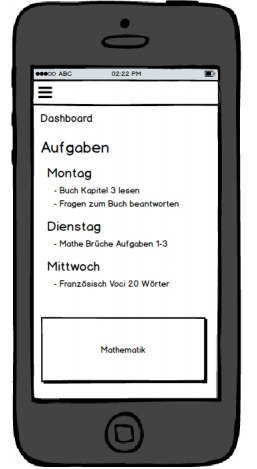
\includegraphics[width=5cm, keepaspectratio]{images/Mockups/Dashboard_Smartphone.png}
		\caption{Mockup Smartphone Dashboard}
	\end{figure}
\end{minipage}


\subsubsection*{Struktur}
Die Aufgabe dieser Seite ist es, neue Aufgaben und Fragen zu definieren. Mit dem Risiko die Seite zu überladen, dem Benutzer jedoch eine bessere Übersicht zu bieten, wurde ein Kompromiss eingegangen und entschieden, dass auch die dazugehörenden Hilfestellungen erfasst werden können. \\

\begin{minipage}{\textwidth}
	\begin{figure}[H]
	\centering
		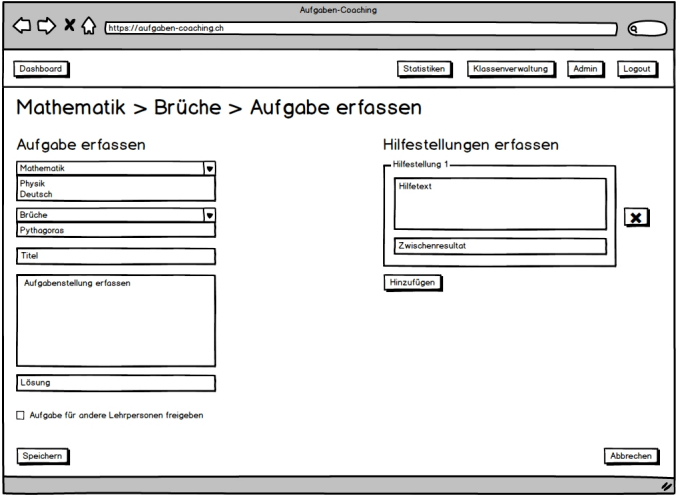
\includegraphics[width=\textwidth, keepaspectratio]{images/Mockups/AufgabeErfassen_Desktop.png}
		\caption{Mockup Aufgabe erfassen Desktop}
	\end{figure}
\end{minipage}


\subsubsection*{Navigation}
In der Navigationsbar sind die fünf definierten Bereiche ersichtlich. Dashboard stellt den Schulstoff Bereich dar, Statistiken die Statistiken, Klassenverwaltung die Klassenverwaltung, Admin das Adminpanel und Logout/Login die User. \\

Damit die Navigationsbar auch in der Mobile Version gut benutzbar ist, wird ein Hamburger Menu erstellt. Klickt ein Benutzer darauf, klappt sich die Navigationsbar auf. \\

\begin{minipage}{\textwidth}
	\begin{figure}[H]
	\centering
		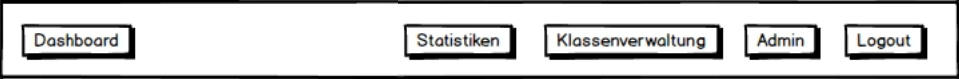
\includegraphics[width=\textwidth, keepaspectratio]{images/Mockups/Navigationsleiste_Desktop.png}
		\caption{Mockup Navigationsbar Desktop}
	\end{figure}
\end{minipage}


\subsubsection*{Orientierung} 
Durch die Breadcrumbs wird hierarchisch dargestellt, wo sich ein Benutzer aktuell auf der Webseite befindet. Mit einem Klick auf die übergeordneten Bereiche navigiert man auch auf diese. \\

\begin{minipage}{\textwidth}
	\begin{figure}[H]
	\centering
		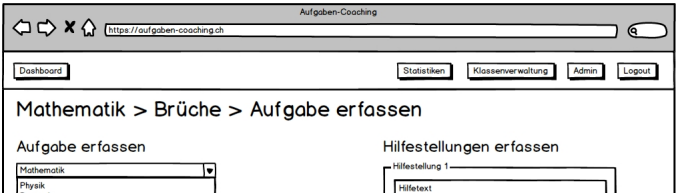
\includegraphics[width=\textwidth, keepaspectratio]{images/Mockups/Breadcrumbs_Desktop.png}
		\caption{Mockup Breadcrumbs Desktop}
	\end{figure}
\end{minipage}


\subsubsection*{Kontrast}
Da die Mockups in schwarz und weiss erstellt wurden, gibt es hierfür kein Beispiel. Die Entscheidung wurde natürlich dennoch in die Entwicklung miteinbezogen.


\newpage